\documentclass{beamer}
\usepackage{amssymb,amsmath,amsthm}
\usepackage{color}
\usepackage{subfig}
\usepackage[]{graphicx}
\usepackage[]{bm}
\usepackage{xcolor}
\usepackage[mathscr]{eucal}
\usepackage{epsfig}

\mode<presentation>
{
\usetheme{Ilmenau}
\usecolortheme{beaver}
}

\title{Applications of Structured Learning to Polyphonic Transcription}
\author[]{J. Shi and C. Herrmann}
\institute[]{Presented for Advanced Topics in Machine Learning}

\makeindex

\begin{document}
\begin{frame}{}
\titlepage
Using structured learning to transcribe piano music
\end{frame}

\section{Motivation}
% 1 minute; total: 1
\begin{frame}{Example}
%Please listen to the following selections.
\end{frame}

% 1 minute; total: 2

\begin{frame}{The Problem}

\only<1-1>{
  {\bf Goal:} Given a recording of a song, transcribe the song in an accurate manner.\\
  \vspace{.5cm}
  {\bf Input:} Recording of song taken in variable settings and with variable quality of recording equipment.\\
  \vspace{.1cm}
  {\bf Output:} MIDI file of the song.
}
\only<2-2>{
  % Be sure to mention overtones and point out disappearing partials.
  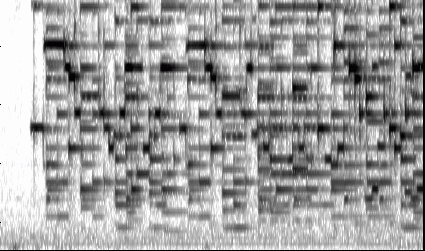
\includegraphics[width=\textwidth]{spectogram.png}
}
\end{frame}

% 1 minute; total: 3
\section{Previous Solutions}
\begin{frame}{Previous Solutions}

General approach:

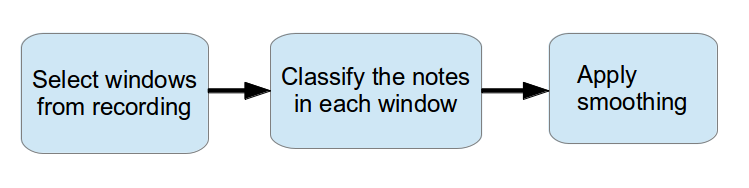
\includegraphics[scale=.4]{algorithm_template.png}

Some separate the classification of notes into two steps: note onset detection and then classification of tones. These tend to suffer, why?
\end{frame}

% 1 minute; total: 4
\begin{frame}{Previous Solutions}
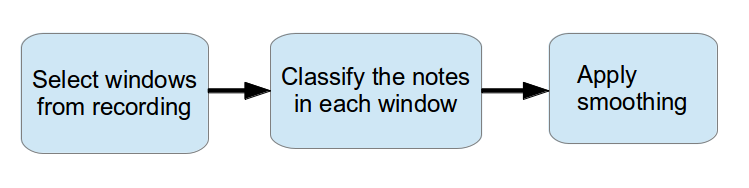
\includegraphics[scale=.4]{algorithm_template.png}

\begin{itemize}
\item How to select the windows? Overlapping? Multiple windows with different lengths?
\item What classification technique to use? How to extract feature vector from windows?
\item What smoothing technique should be applied? How much should this encompass.
\end{itemize}
\end{frame}

% 1 minute; total: 5
\begin{frame}{Previous Solutions}
\begin{description} 
\item[Discriminative] \hfill \\ 
    \begin{itemize}\setlength{\itemindent}{-5em}
    \item  Uses SVM one-versus-all classifiers.
    \end{itemize}
\item[Generative/Recursive Neural Nets] \hfill \\
    \begin{itemize}\setlength{\itemindent}{-5em}
    \item Uses neural nets to generate features,
    \item or models ``listening'' using stateful oscillators.
    \end{itemize}
\item[F0 approach] \hfill \\
    \begin{itemize}\setlength{\itemindent}{-5em}
    \item Repeatedly detects and subtracts the predominant note,
    \item or uses E-M with frequency profiles for each possible note.
    \end{itemize}
\end{description}
\end{frame}

% 1 minute; total: 6
\section{Algorithm}
\begin{frame}{Idea}
So far the discriminative approaches have performed the best.\\
\vspace{.5cm}

\pause
A couple of thoughts:
\begin{itemize}
\item One-versus-All SVM is terrible!
\item Can improve the feature vectors chosen and the way windowing is done.
\item Why emphasis on the HMM at end? % make sure to explain which HMM?
\end{itemize}
\end{frame}

% 1 minute; total: 7
\begin{frame}{New System}
Structural SVM. Find the $arg\,max_{x} f(x,y)$.

\vspace{1em}
Markov model of correlations:
\begin{itemize}
\item between notes played at the same time.
\item between notes played in the present vs. past/future.
\end{itemize}

\vspace{1em}
Features: spectograms.
\end{frame}

% 1 minute; total: 8
\begin{frame}{Benefits}
Smoothing included in classification.

\vspace{1em}
Classification of onsets/offsets.

\vspace{1em}
Using differences across adjacent time steps in onset/offset classification.
\end{frame}

% 1 minute; total: 9
\section{Preliminary Results}
\begin{frame}{Preliminary Results}
On simple chords
\begin{itemize}
\item Multiclass performs better than OvA classifier
\item Structured performs better than multiclass
\end{itemize}

On start of music with super limited HMM smoothing
\begin{itemize}
\item Multiclass performs better than OvA classifier
\item Structured performs very slightly better than multiclass. Still in progress!
\end{itemize}
\end{frame}

% 0.5 minute; total: 9.5
\section{Summary}
\begin{frame}{Summary}
Seems like we can improve on state of the art techniques in polyphonic transcription using existing structured learning techniques. 
\end{frame}
\end{document}
